\section{Thiết kế mockup UI cho hệ thống}
    \subsection{Trang đăng nhập}
        \begin{figure}[h]
            \centering
            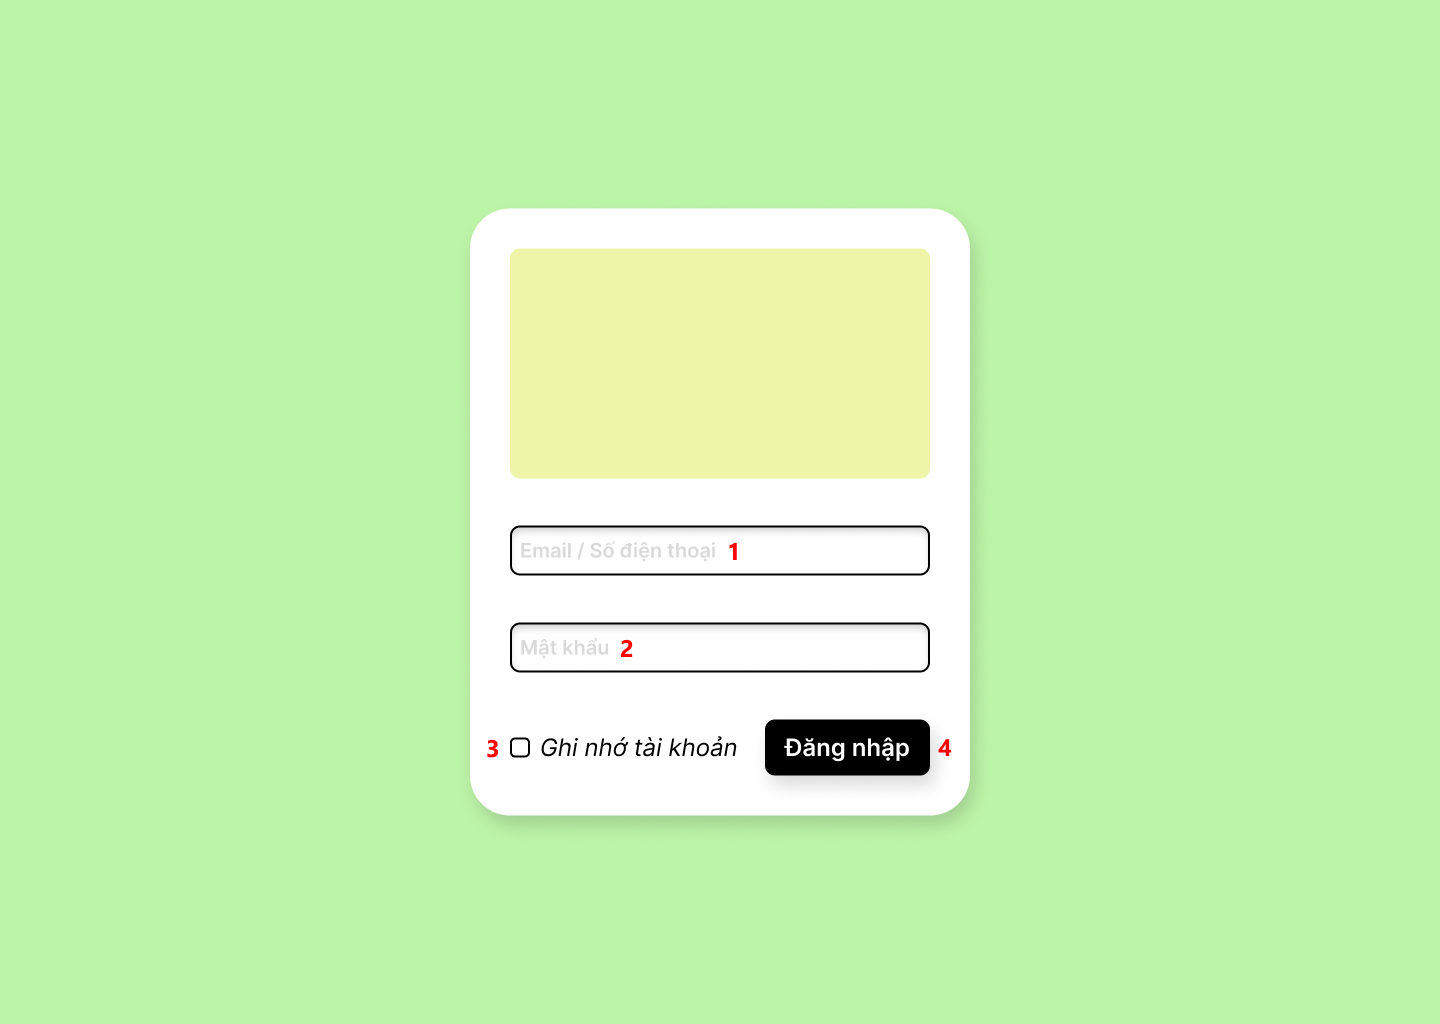
\includegraphics[width=1\linewidth]{imgs/mockup/login.png}
            \caption{UI trang đăng nhập}
        \end{figure}

        \begin{tblr}{
            width=0.9\linewidth,
            hlines, 
            vlines,
            colspec={X[-1]X[2]X[7]},
            columns = {valign = m, },
            column{1} = {halign = c},
            row{1} = {halign = c, valign = m, bg = lightgray, fg = black},
            }
            {\textbf{\#}} & \textbf{Type} & {\textbf{Mô tả}} \\
            1 & Input & Người dùng nhập email / số điện thoại\\
            2 & Input &  Người dùng nhập password\\
            3 & Check box & Lưu tài khoản của người dùng\\
            4 & Button & Xác nhận đăng nhập \newline
                         Hệ thống kiểm tra, nếu đúng \newline
                          - Chuyển sang trang công việc hôm nay nếu là worker \newline
                          - Chuyển sang trang MCP nếu là back officer\\
        \end{tblr}
        \newpage

    \subsection{Hiển thị menu chính của worker}
        \begin{figure}[h]
            \centering
            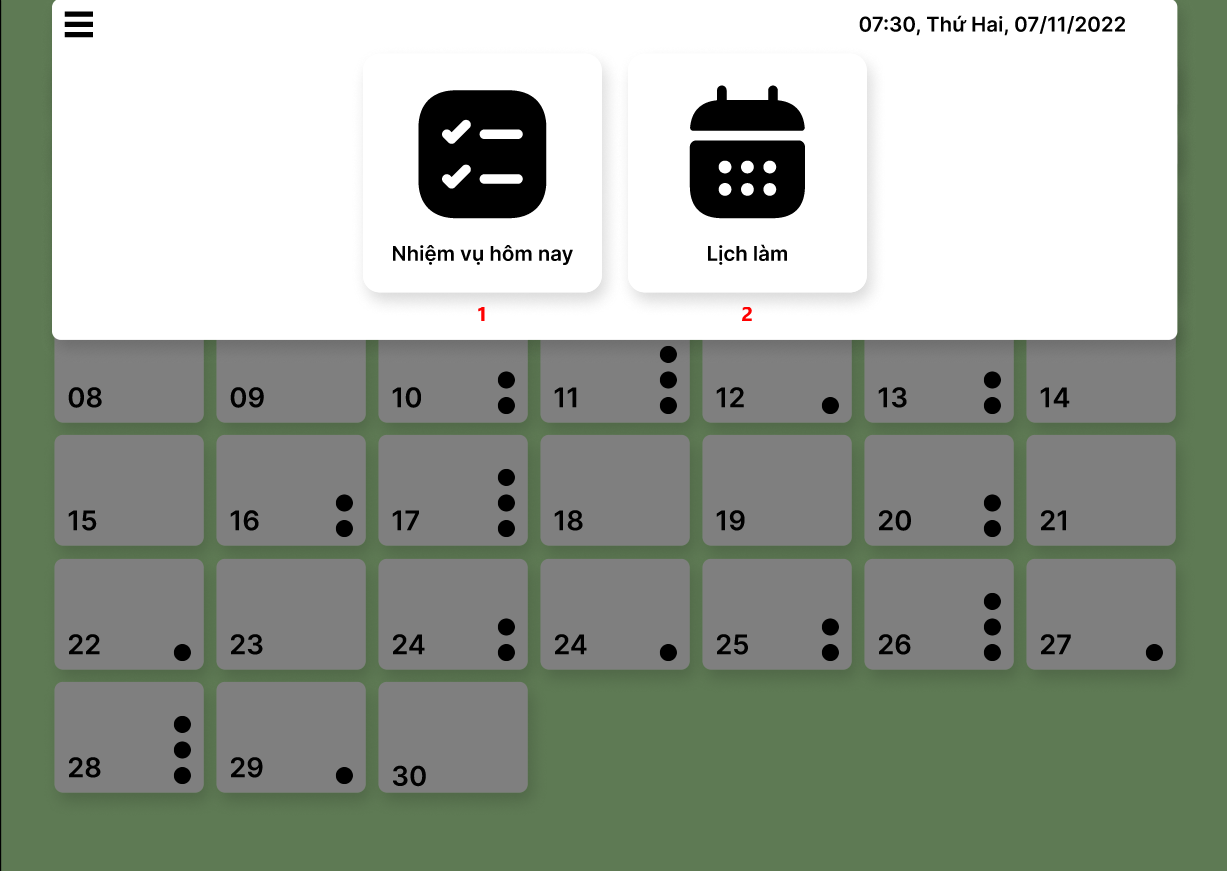
\includegraphics[width=1\linewidth]{imgs/mockup/worker main menu.png}
            \caption{UI menu chính của worker}
        \end{figure}

        \begin{tblr}{
            width=0.9\linewidth,
            hlines, 
            vlines,
            colspec={X[-1]X[1]X[7]},
            columns = {valign = m, },
            column{1} = {halign = c},
            row{1} = {halign = c, valign = m, bg = lightgray, fg = black},
            }
            {\textbf{\#}} & \textbf{Type} & {\textbf{Mô tả}} \\
            1 & Button & Chuyển tới trang công việc hôm nay\\
            2 & Button &  Chuyển tới trang lịch làm việc\\
        \end{tblr}
        \newpage
    
    \subsection{Hiển thị menu chính của back officer}
        \begin{figure}[h]
            \centering
            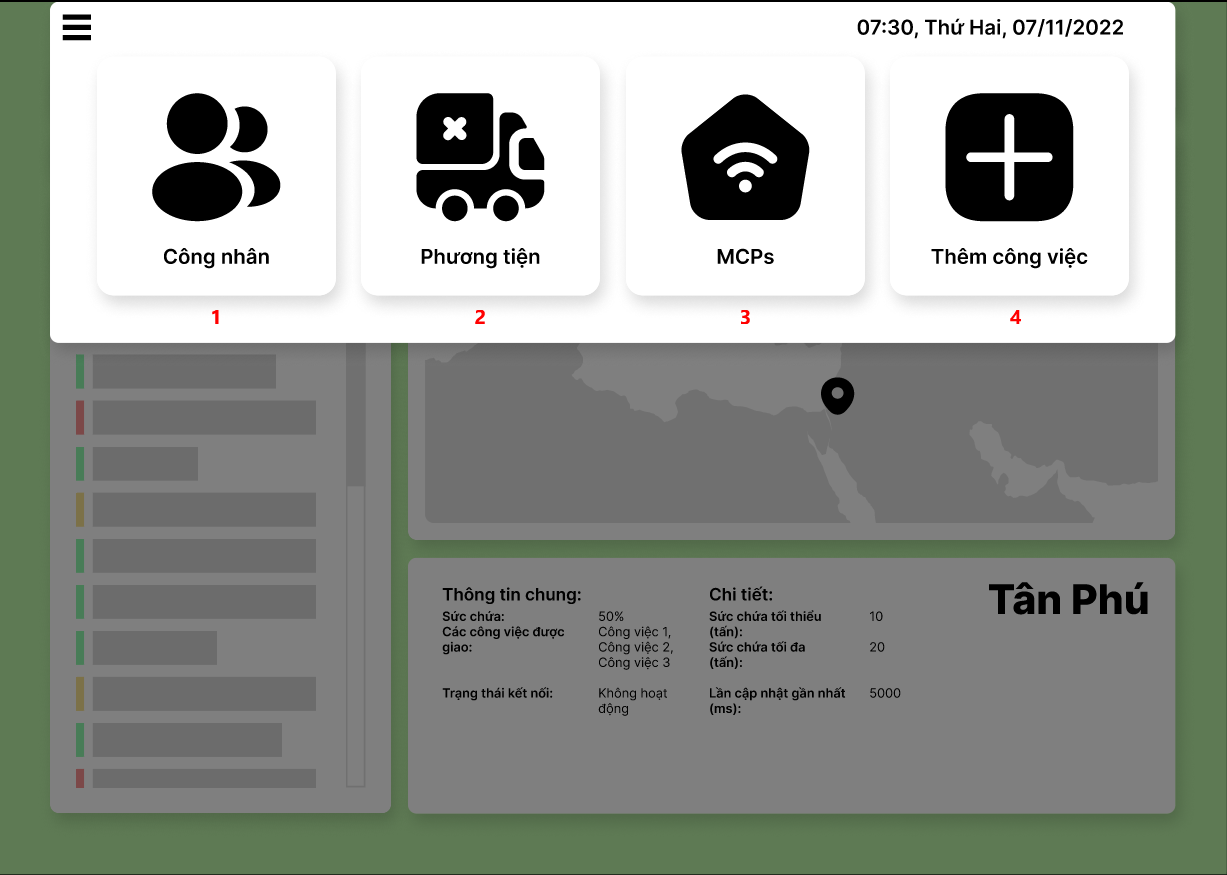
\includegraphics[width=1\linewidth]{imgs/mockup/main menu.png}
            \caption{UI menu chính của back officer}
        \end{figure}

        \begin{tblr}{
            width=0.9\linewidth,
            hlines, 
            vlines,
            colspec={X[-1]X[1]X[7]},
            columns = {valign = m, },
            column{1} = {halign = c},
            row{1} = {halign = c, valign = m, bg = lightgray, fg = black},
            }
            {\textbf{\#}} & \textbf{Type} & {\textbf{Mô tả}} \\
            1 & Button & Chuyển sang trang quản lý công nhân\\
            2 & Button & Chuyển sang trang quản lý phương tiện\\
            3 & Button & Chuyển sang trang quản lý MCP\\
            4 & Button & Chuyển sang trang tạo công việc mới\\
        \end{tblr}
        \newpage

    \subsection{Hiển thị menu tài khoản}
        \begin{figure}[h]
            \centering
            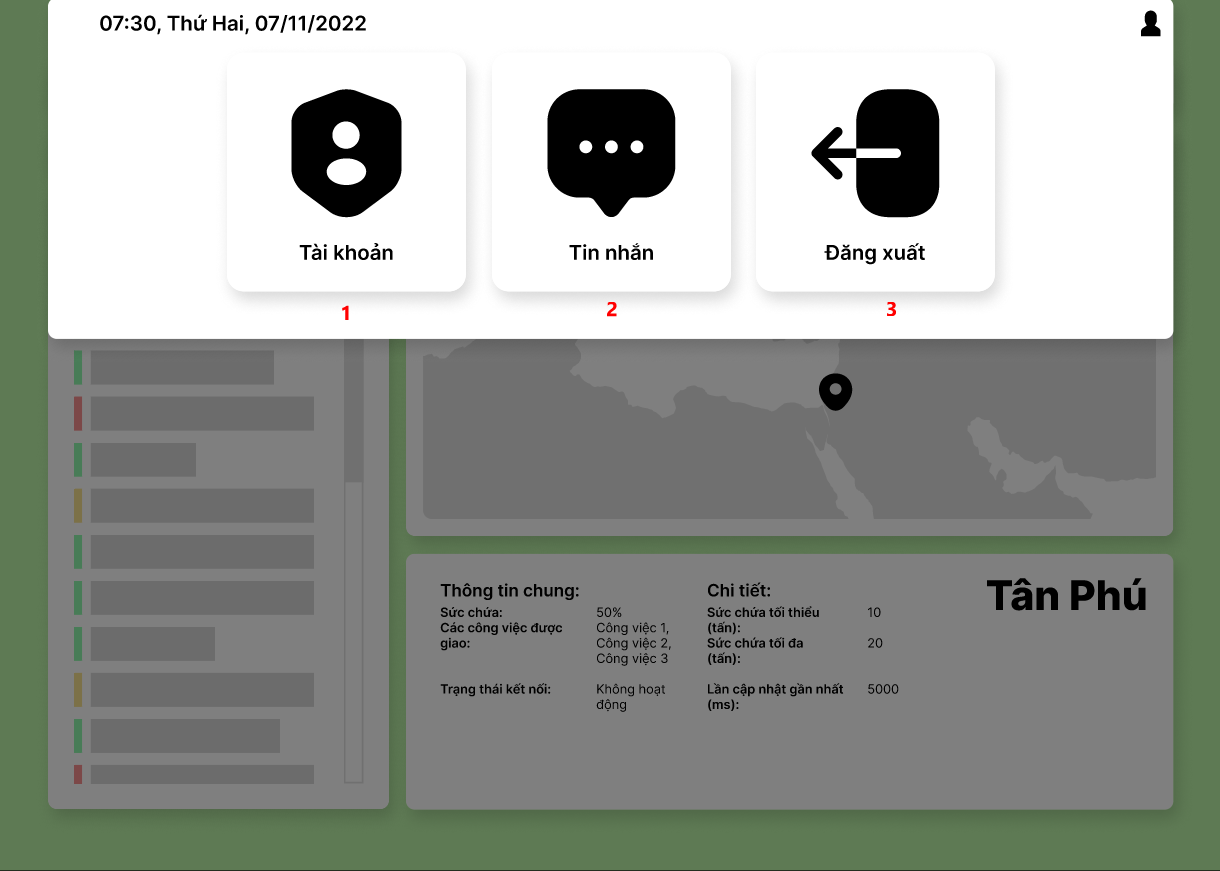
\includegraphics[width=1\linewidth]{imgs/mockup/account menu.png}
            \caption{UI hiển thị menu tài khoản}
        \end{figure}

        \begin{tblr}{
            width=0.9\linewidth,
            hlines, 
            vlines,
            colspec={X[-1]X[1]X[7]},
            columns = {valign = m, },
            column{1} = {halign = c},
            row{1} = {halign = c, valign = m, bg = lightgray, fg = black},
            }
            {\textbf{\#}} & \textbf{Type} & {\textbf{Mô tả}} \\
            1 & Button & Chuyển sang trang thông tin cá nhân\\
            2 & Button & Chuyển sang trang nhắn tin\\
            3 & Button & Đăng xuất và chuyển sang trang đăng nhập
        \end{tblr}
        \newpage

    \subsection{Trang công việc hôm nay}
        \begin{figure}[h]
            \centering
            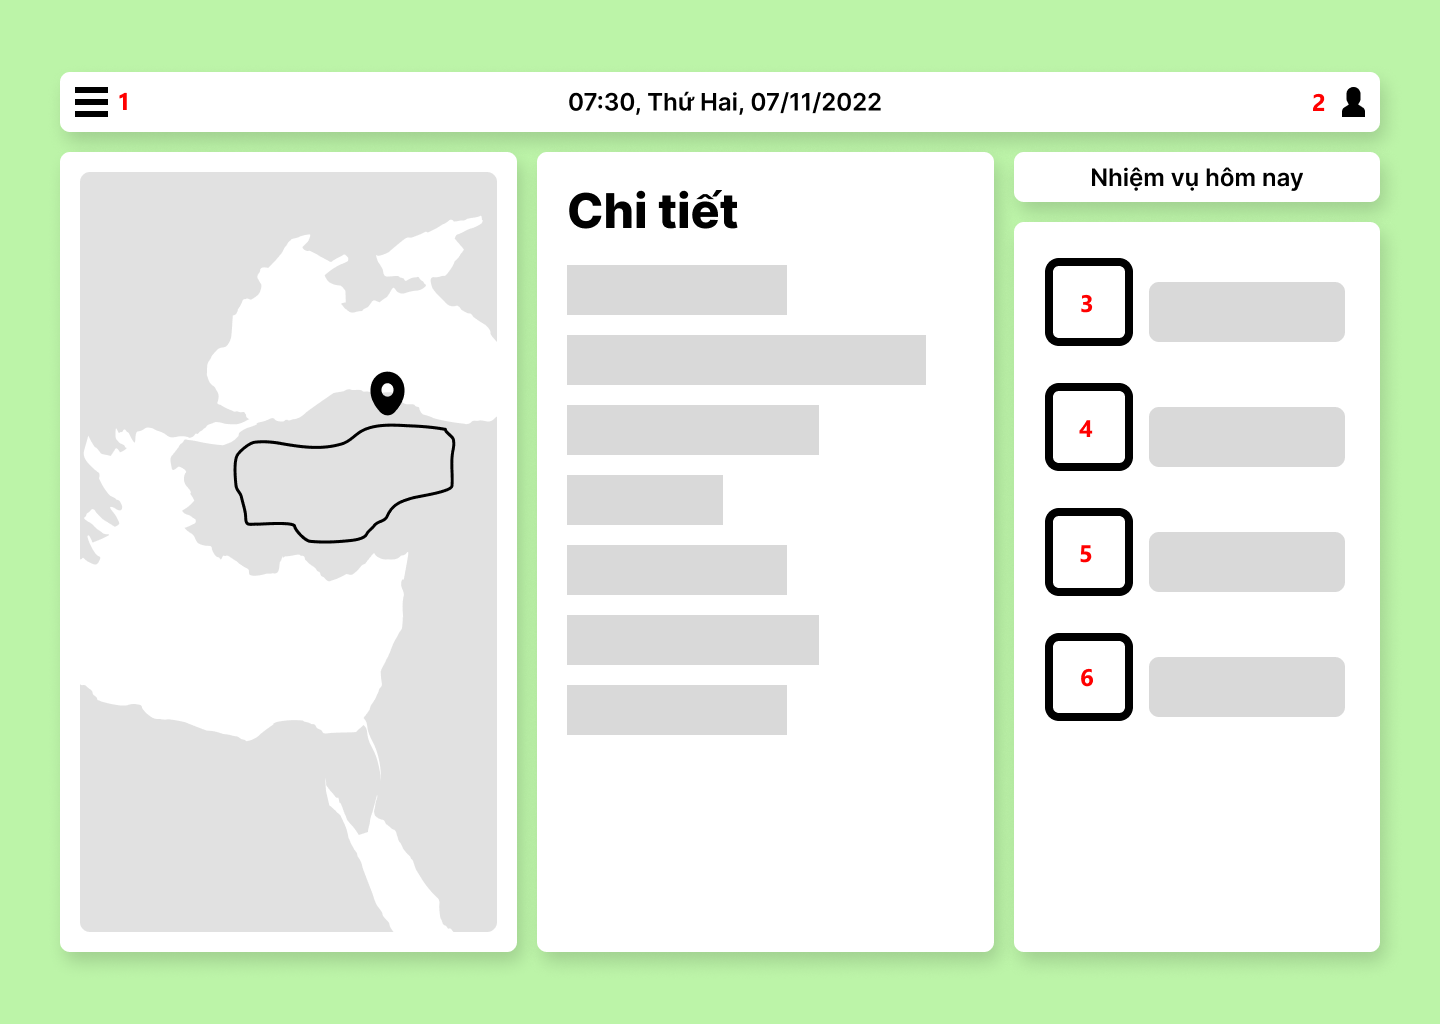
\includegraphics[width=1\linewidth]{imgs/mockup/today's task.png}
            \caption{UI trang công việc hôm nay}
        \end{figure}

        \begin{tblr}{
            width=0.9\linewidth,
            hlines, 
            vlines,
            colspec={X[-1]X[2]X[7]},
            columns = {valign = m, },
            column{1} = {halign = c},
            row{1} = {halign = c, valign = m, bg = lightgray, fg = black},
            }
            {\textbf{\#}} & \textbf{Type} & {\textbf{Mô tả}} \\
            1 & Button & Hiển thị menu chính\\
            2 & Button &  Hiển thị menu tài khoản\\
            3,4,5,6 & Check box & Đánh dâu công việc đã hoàn thành\\
        \end{tblr}
        \newpage
    
    \subsection{Trang lịch làm việc}
        \begin{figure}[h]
            \centering
            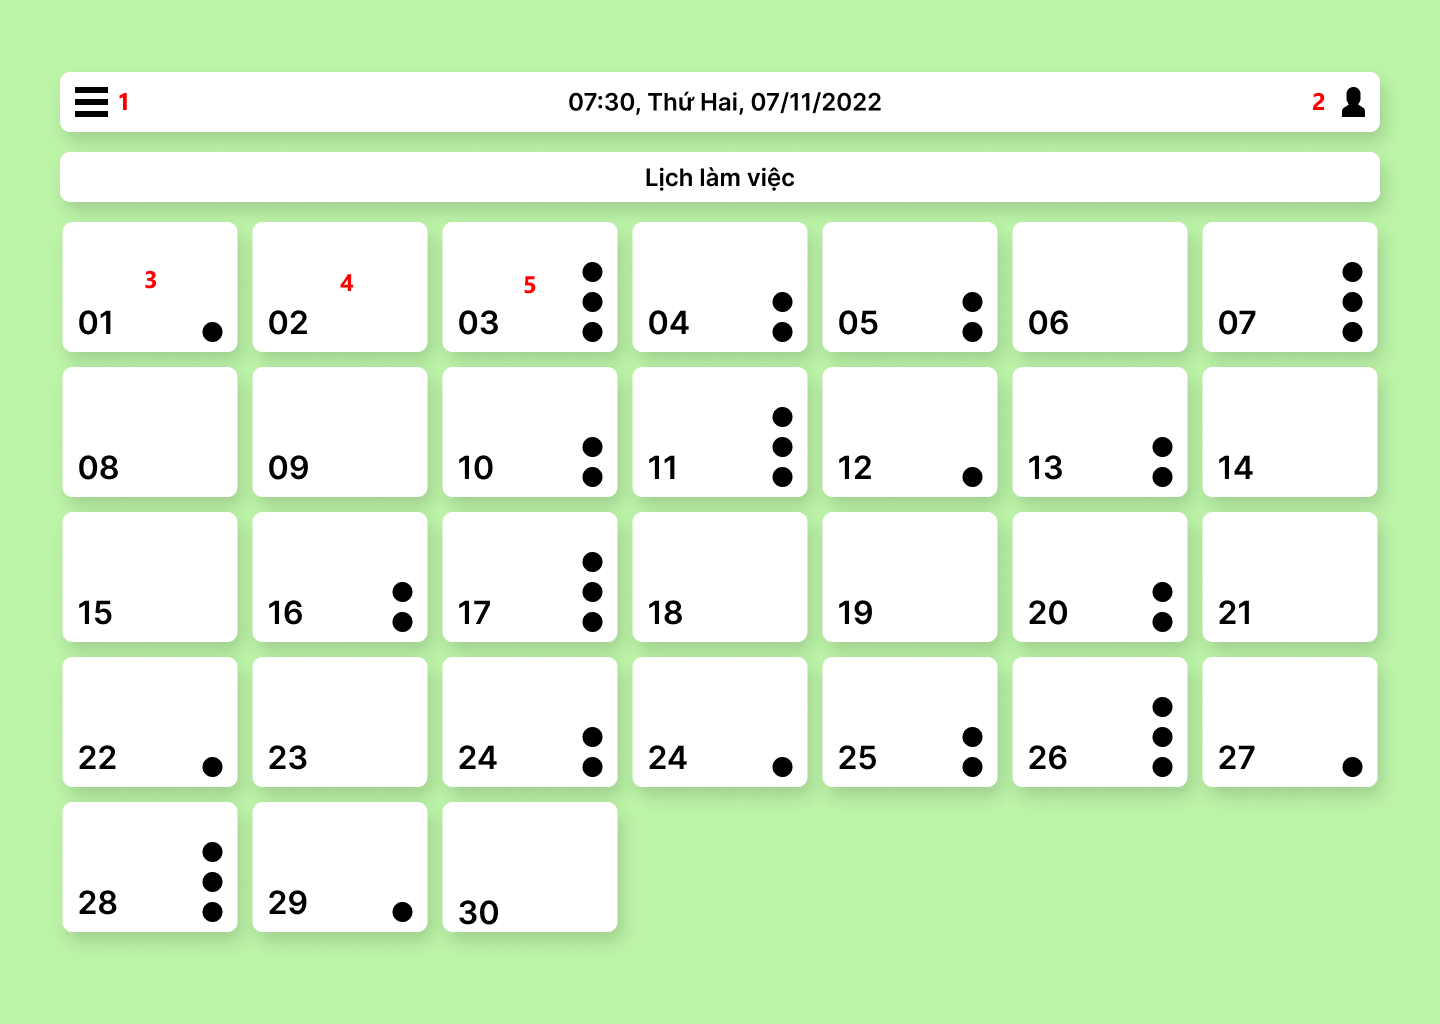
\includegraphics[width=0.7\textwidth]{imgs/mockup/work calendar.png} % first figure itself
            \caption{UI trang lịch làm việc}
        \end{figure}

        \begin{figure}[h]
            \centering
                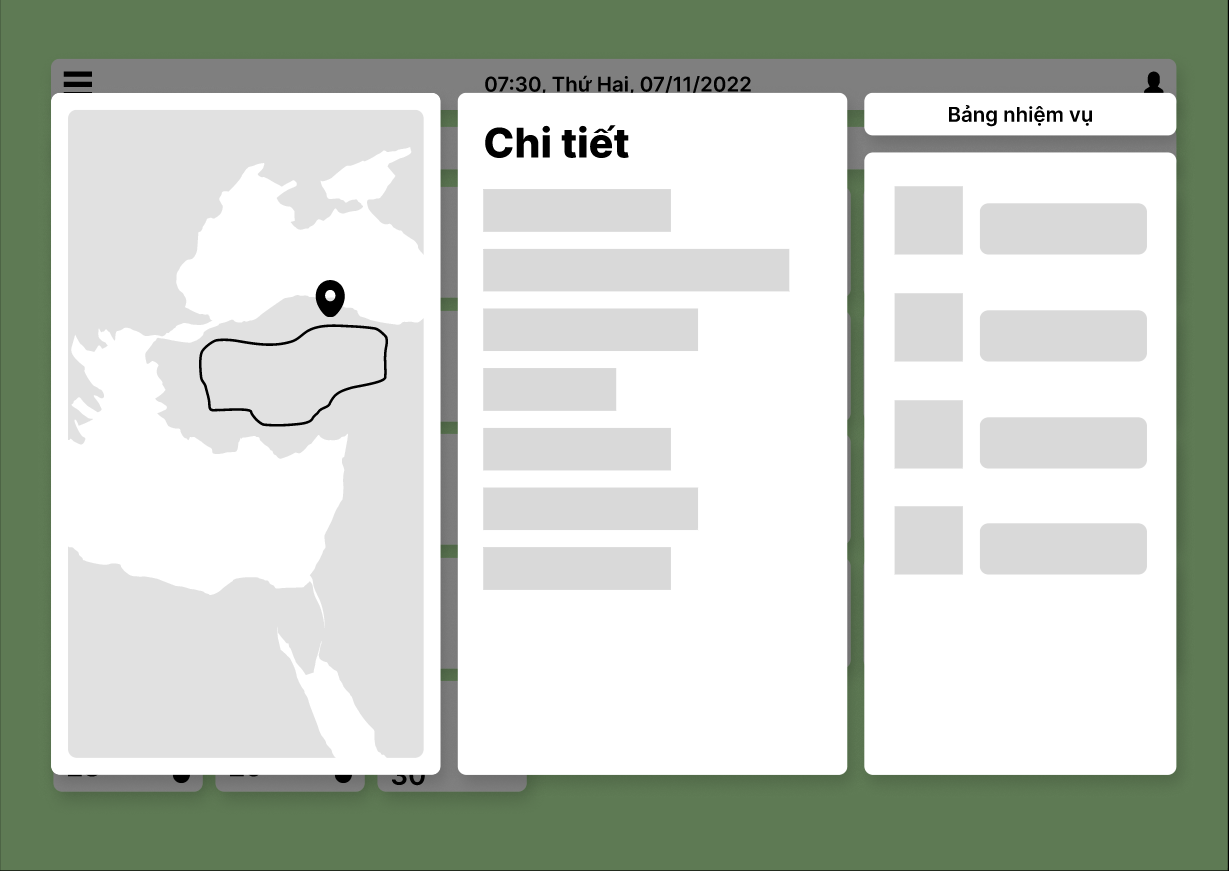
\includegraphics[width=0.6\textwidth]{imgs/mockup/work calendar task detail.png} % second figure itself
                \caption{UI phần hiển thị chi tiết công việc trong ngày được chọn}
        \end{figure}

        \begin{tblr}{
            width=0.9\linewidth,
            hlines, 
            vlines,
            colspec={X[-1]X[1]X[7]},
            columns = {valign = m, },
            column{1} = {halign = c},
            row{1} = {halign = c, valign = m, bg = lightgray, fg = black},
            }
            {\textbf{\#}} & \textbf{Type} & {\textbf{Mô tả}} \\
            1 & Button & Hiển thị menu chính\\
            2 & Button & Hiển thị menu tài khoản\\
            3,4,5 & Button & Hiển thị chi tiết công việc trong ngày được chọn\\
        \end{tblr}
        \newpage
    
    \subsection{Trang thông tin cá nhân}
        \begin{figure}[h]
            \centering
            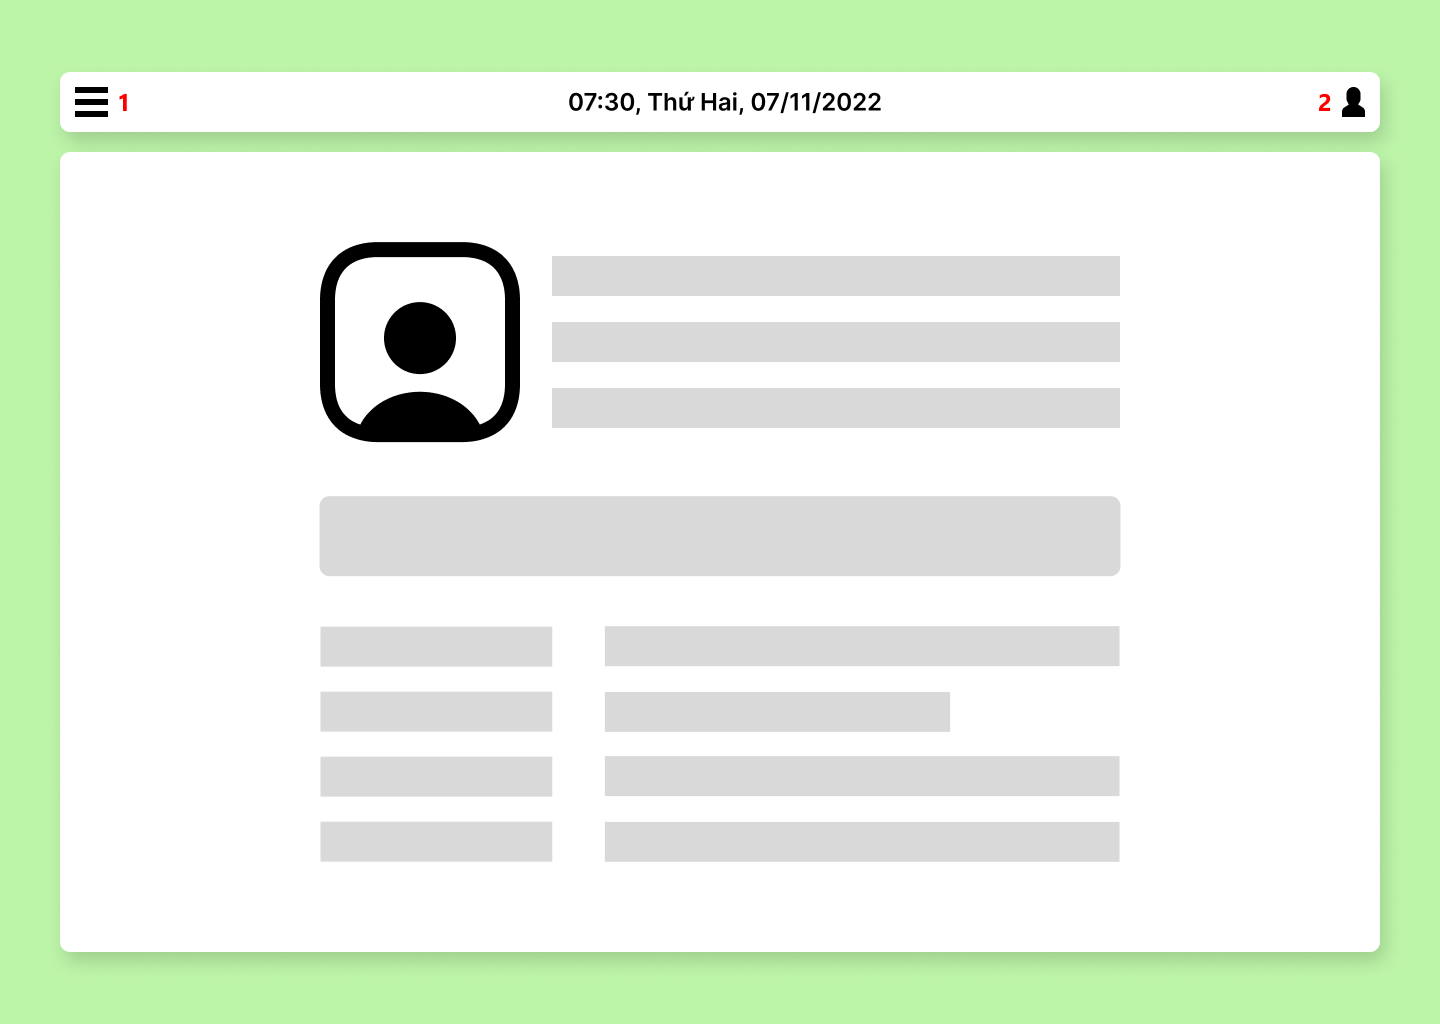
\includegraphics[width=1\textwidth]{imgs/mockup/Profile.png} % first figure itself
            \caption{UI trang thông tin cá nhân}
        \end{figure}

        \begin{tblr}{
            width=0.9\linewidth,
            hlines, 
            vlines,
            colspec={X[-1]X[1]X[7]},
            columns = {valign = m, },
            column{1} = {halign = c},
            row{1} = {halign = c, valign = m, bg = lightgray, fg = black},
            }
            {\textbf{\#}} & \textbf{Type} & {\textbf{Mô tả}} \\
            1 & Button & Hiển thị menu chính\\
            2 & Button & Hiển thị menu tài khoản\\
        \end{tblr}
        \newpage

    \subsection{Trang nhắn tin}
        \begin{figure}[h]
            \centering
            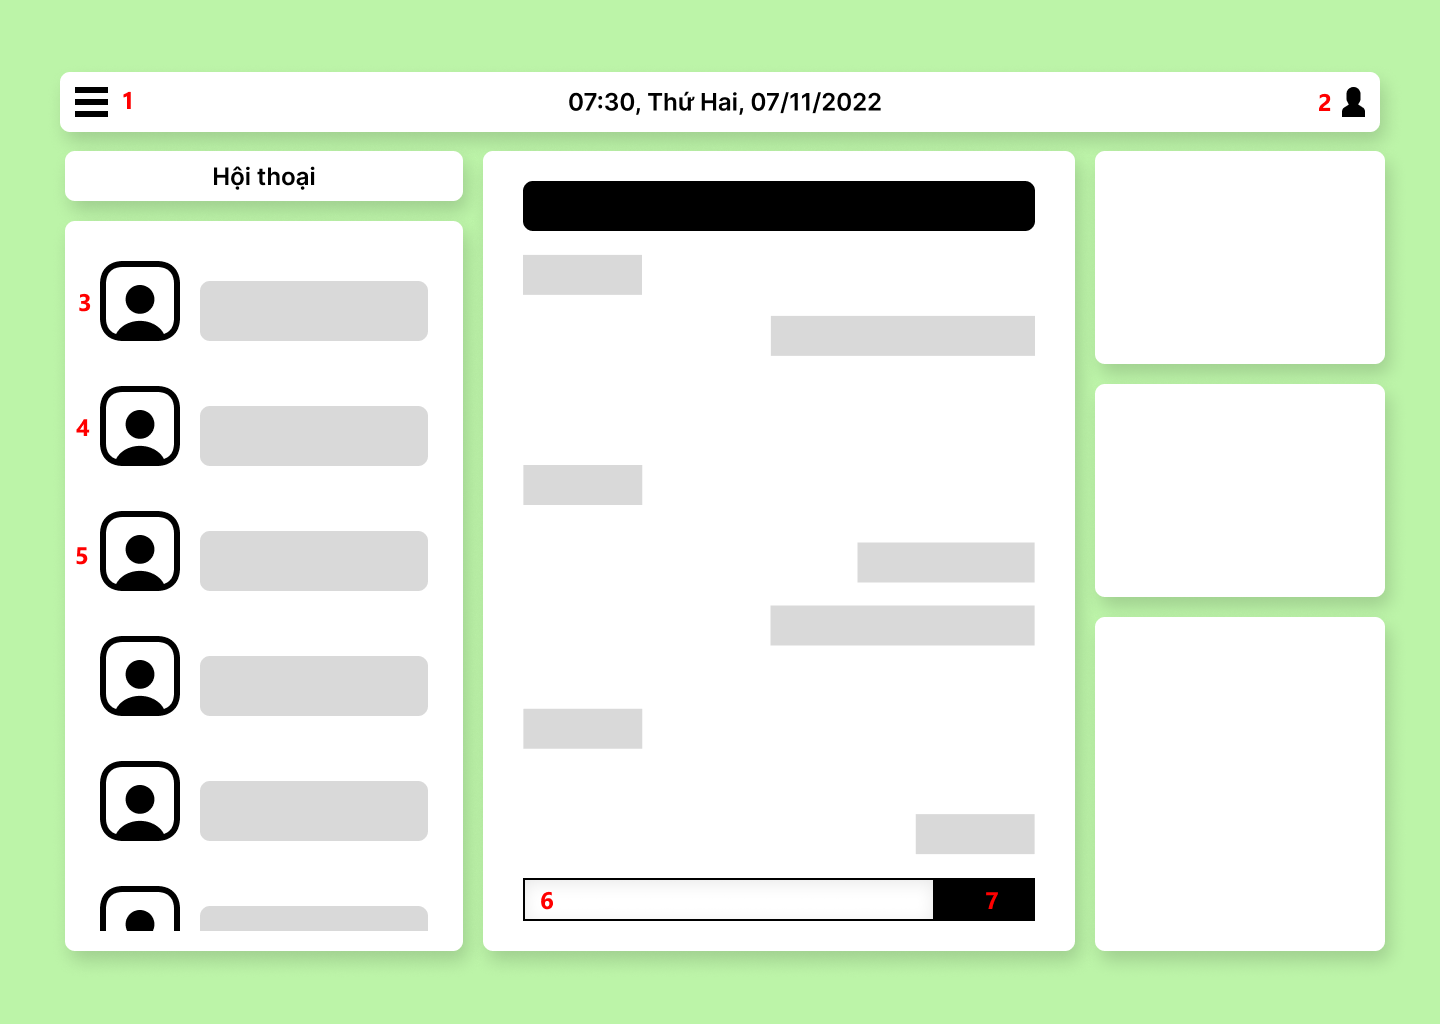
\includegraphics[width=1\linewidth]{imgs/mockup/chat.png}
            \caption{UI trang nhắn tin}
        \end{figure}

        \begin{tblr}{
            width=0.9\linewidth,
            hlines, 
            vlines,
            colspec={X[-1]X[1]X[7]},
            columns = {valign = m, },
            column{1} = {halign = c},
            row{1} = {halign = c, valign = m, bg = lightgray, fg = black},
            }
            {\textbf{\#}} & \textbf{Type} & {\textbf{Mô tả}} \\
            1 & Button & Hiển thị menu chính\\
            2 & Button & Hiển thị menu phụ\\
            3,4,5 & List & Chọn nhân viên muốn nhắn tin, phần tin nhắn sẽ hiển thi bên phải\\
            6 & Input & Nhập tin nhắn\\
            7 & Button & Gửi tin nhắn \\
        \end{tblr}
        \newpage

    \subsection{Trang MCPs}
        \begin{figure}[h]
            \centering
            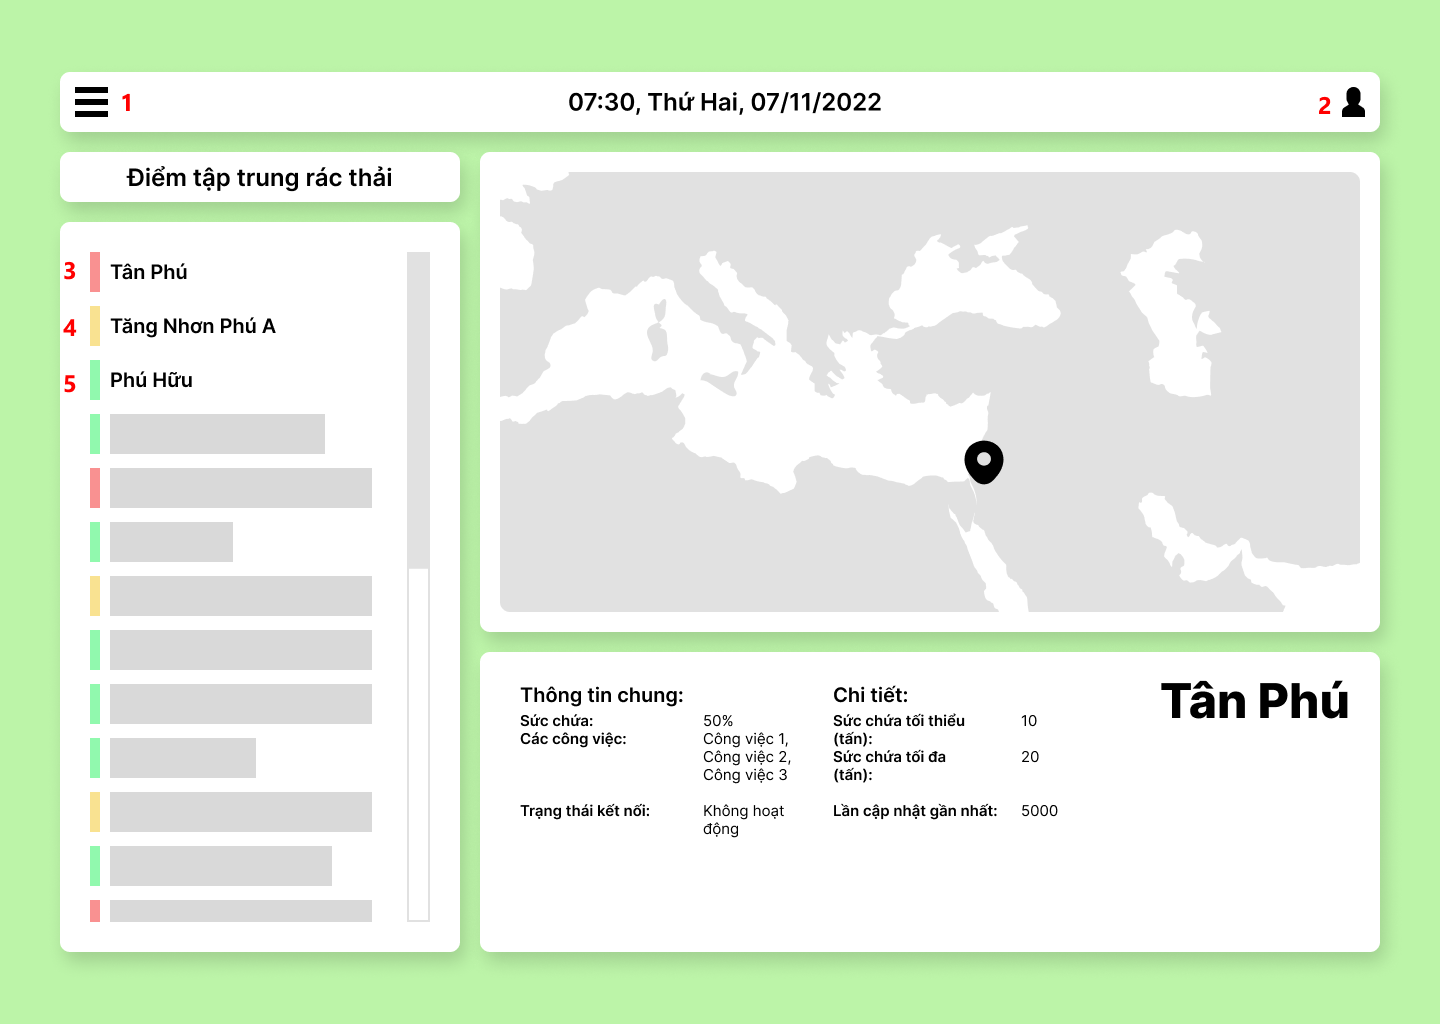
\includegraphics[width=1\linewidth]{imgs/mockup/MCP status.png}
            \caption{UI trang thông tin MCP}
        \end{figure}

        \begin{tblr}{
            width=0.9\linewidth,
            hlines, 
            vlines,
            colspec={X[-1]X[1]X[7]},
            columns = {valign = m, },
            column{1} = {halign = c},
            row{1} = {halign = c, valign = m, bg = lightgray, fg = black},
            }
            {\textbf{\#}} & \textbf{Type} & {\textbf{Mô tả}} \\
            1 & Button & Hiển thị menu chính\\
            2 & Button & Hiển thị menu phụ\\
            3,4,5 & List & Chọn MCP muốn xem, thông tin sẽ được hiển thị bên phải
        \end{tblr}
        \newpage
    
    \subsection{Trang quản lý phương tiện}
        \begin{figure}[h]
            \centering
            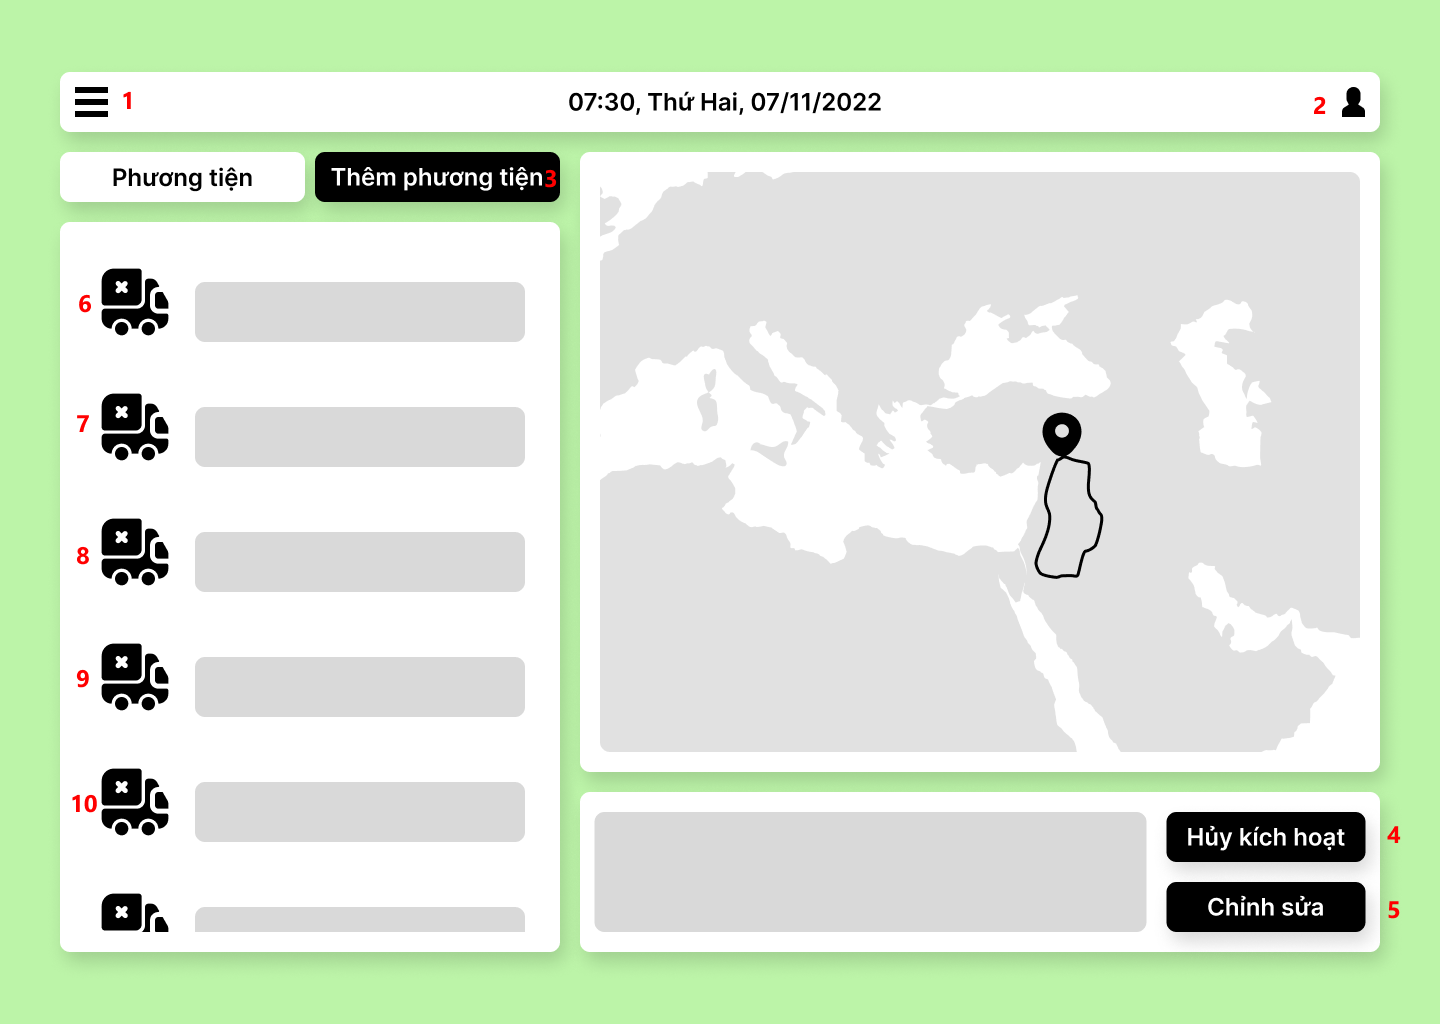
\includegraphics[width=1\linewidth]{imgs/mockup/vehicles.png}
            \caption{UI trang quản lý phương tiện}
        \end{figure}

        \begin{tblr}{
            width=0.9\linewidth,
            hlines, 
            vlines,
            colspec={X[-1]X[1]X[7]},
            columns = {valign = m, },
            column{1} = {halign = c},
            row{1} = {halign = c, valign = m, bg = lightgray, fg = black},
            }
            {\textbf{\#}} & \textbf{Type} & {\textbf{Mô tả}} \\
            1 & Button & Hiển thị menu chính\\
            2 & Button & Hiển thị menu phụ\\
            3 & Button & Hiển thị phần thêm phương tiện \\
            4 & Button & Thực hiện deactive phương tiện, thông báo xác nhận xuất hiện\\
            5 & Button & Hiển thị phần chỉnh sửa phương tiện\\
            6,7,8,9,10 & List & Chọn phương tiện muốn xem và chỉnh sửa, thông tin sẽ được hiển thị bên phải\\
        \end{tblr}
        \newpage

    \subsection{Trang quản lý công nhân}
        \begin{figure}[h]
            \centering
            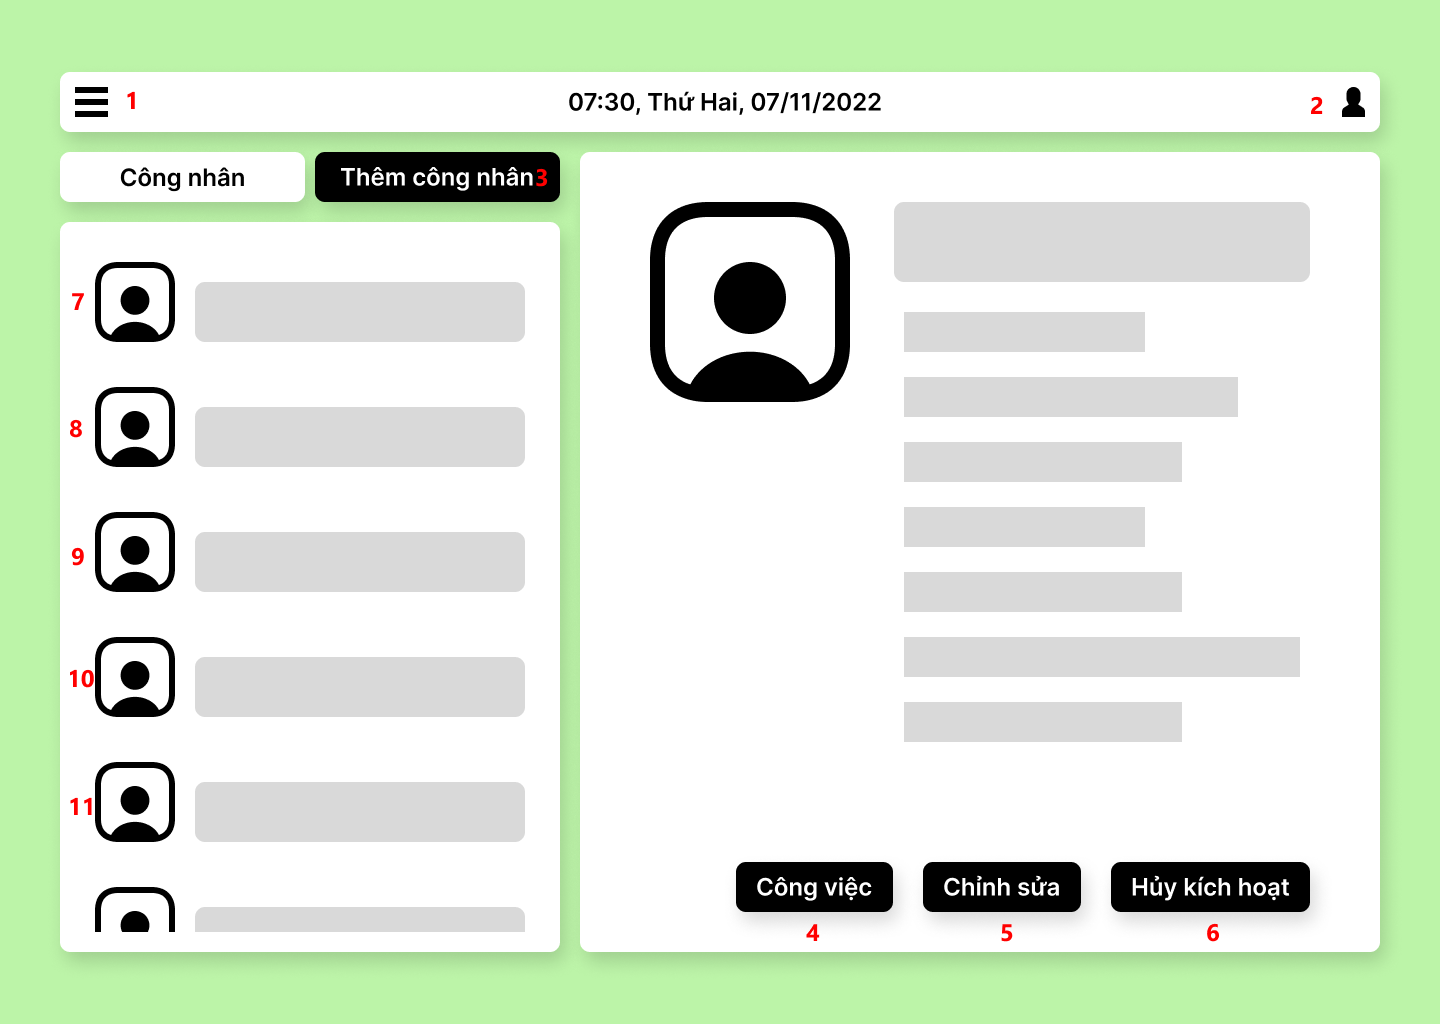
\includegraphics[width=1\linewidth]{imgs/mockup/workers.png}
            \caption{UI trang quản lý công nhân}
        \end{figure}

        \begin{tblr}{
            width=0.9\linewidth,
            hlines, 
            vlines,
            colspec={X[-1]X[1]X[7]},
            columns = {valign = m, },
            column{1} = {halign = c},
            row{1} = {halign = c, valign = m, bg = lightgray, fg = black},
            }
            {\textbf{\#}} & \textbf{Type} & {\textbf{Mô tả}} \\
            1 & Button & Hiển thị menu chính\\
            2 & Button & Hiển thị menu phụ\\
            3 & Button & Hiển thị trang thêm công nhân mới\\
            4 & Button & Xem công việc của công nhân\\
            5 & Button & Hiển thị trang chỉnh sửa công nhân\\
            6 & Button & Thực hiện deactive phương tiện, thông báo xác nhận xuất hiện\\
            7,8,9,\newline 10,11 & List & Chọn công nhân muốn xem và chỉnh sửa, thông tin sẽ được hiển thị bên phải\\
        \end{tblr}
        \newpage

    \subsection{UI phần thêm/sửa công nhân hoặc phương tiện}
        \begin{figure}[h]
            \centering
            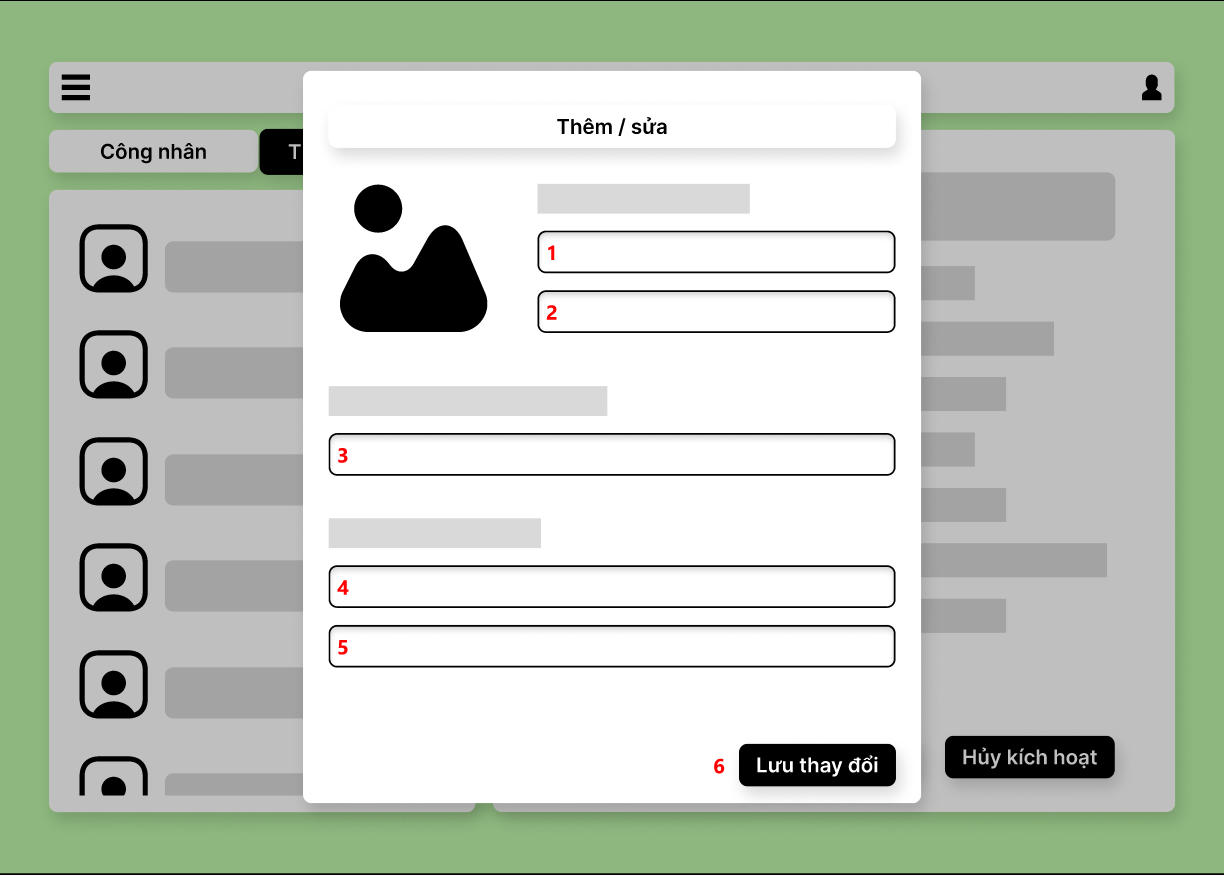
\includegraphics[width=1\linewidth]{imgs/mockup/add_edit.png}
            \caption{UI phần thêm/chỉnh sửa}
        \end{figure}

        \begin{tblr}{
            width=0.9\linewidth,
            hlines, 
            vlines,
            colspec={X[-1]X[1]X[7]},
            columns = {valign = m, },
            column{1} = {halign = c},
            row{1} = {halign = c, valign = m, bg = lightgray, fg = black},
            }
            {\textbf{\#}} & \textbf{Type} & {\textbf{Mô tả}} \\
            1,2,3,4,5 & Input & Nhập các thông tin cần thiết\\
            6 & Button & thực hiện tạo/sửa, thông báo xác nhận xuất hiện\\
        \end{tblr}
        \newpage

    \subsection{UI trang tạo công việc}
        \begin{figure}[h]
            \centering
            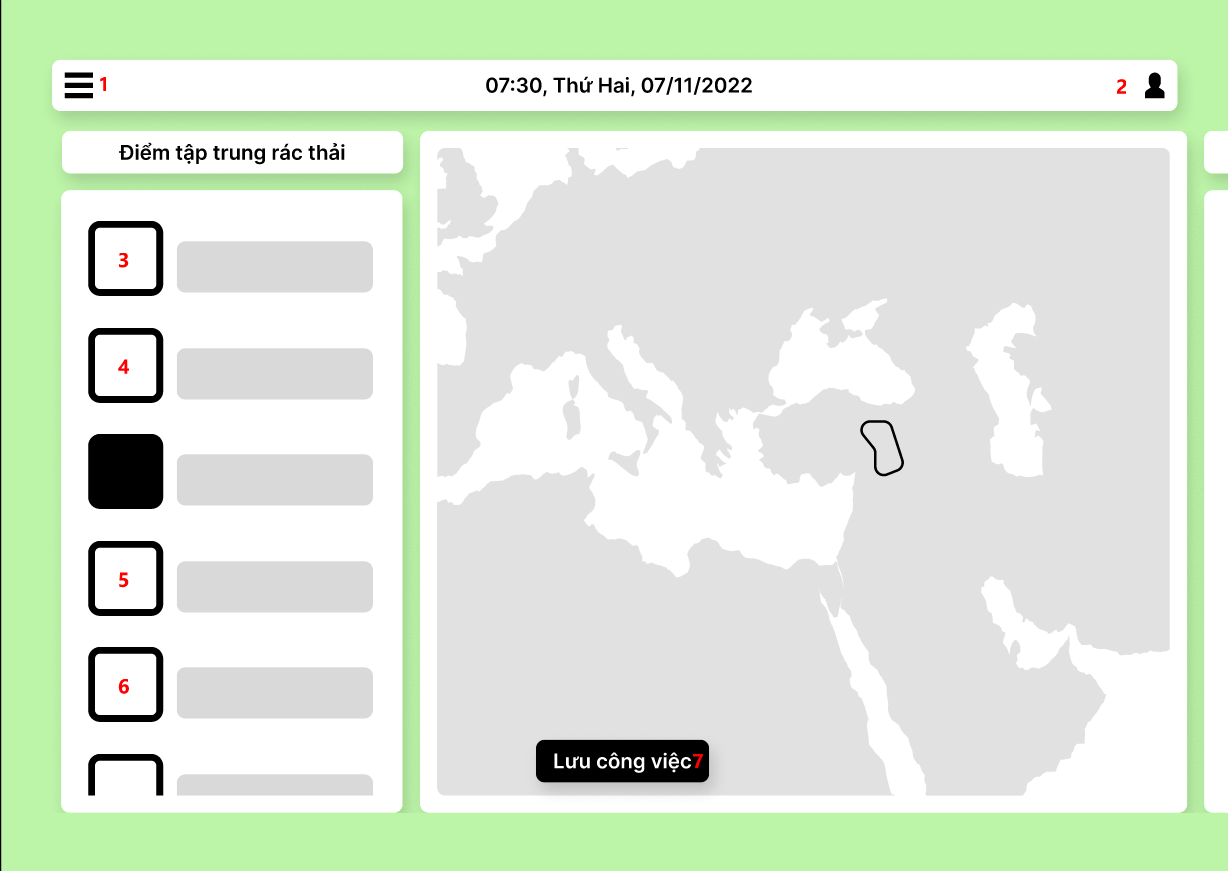
\includegraphics[width=0.6\linewidth]{imgs/mockup/assign task 1.png}
            \caption{UI trang tạo công việc}
        \end{figure}
        \begin{figure}[h]
            \centering
            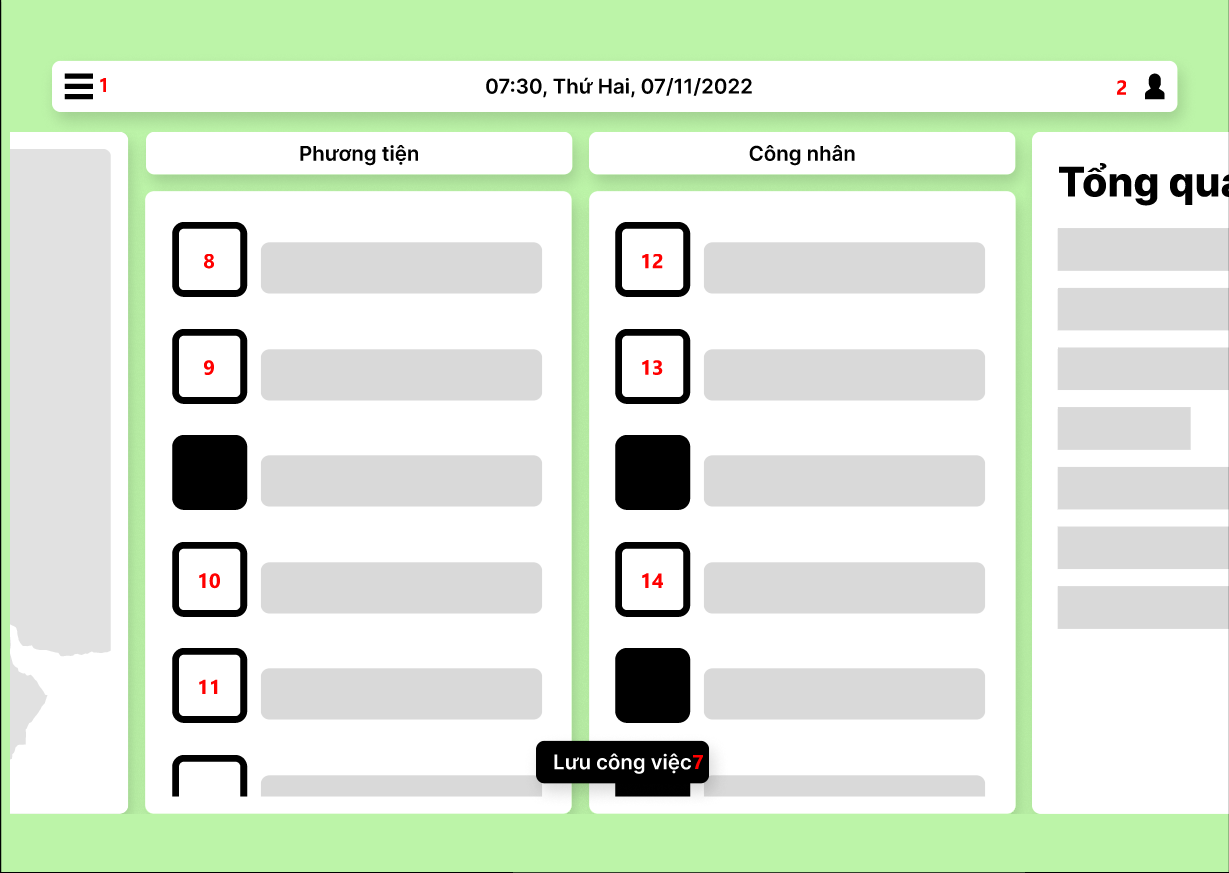
\includegraphics[width=0.6\linewidth]{imgs/mockup/assign task 2.png}
            \caption{UI trang tạo công việc}
        \end{figure}
        
        \begin{tblr}{
            width=0.9\linewidth,
            hlines, 
            vlines,
            colspec={X[-1]X[2]X[7]},
            columns = {valign = m, },
            column{1} = {halign = c},
            row{1} = {halign = c, valign = m, bg = lightgray, fg = black},
            }
            {\textbf{\#}} & \textbf{Type} & {\textbf{Mô tả}} \\
            1 & Button & Hiển thị menu chính\\
            2 & Button & Hiển thị menu phụ\\
            3,4,5,6 & Checkbox & Chọn các điểm MCP \\
            8,9,10,11 & Checkbox & Chọn các phương tiện \\
            12,13,14 & Checkbox & Chọn công nhân \\
            7 & Button & Xác nhận và tạo công việc mới \\
        \end{tblr}
        \newpage

    \subsection{UI thông báo xác nhận}
        \noindent \begin{minipage}{0.5\textwidth}
            \vspace{1cm}
            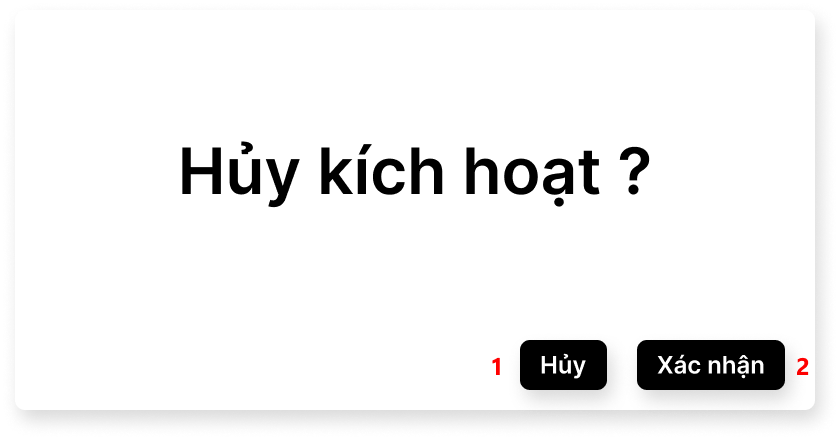
\includegraphics[width=\textwidth]{imgs/mockup/Confirmation pop-up deactive.png}
            \captionof{figure}{UI trang quản lý công nhân}
        \end{minipage}
        \hspace{0.05\textwidth}
        \begin{minipage}{0.45\textwidth}
            \begin{tblr}{
                width=1\linewidth,
                hlines, 
                vlines,
                colspec={X[-1]X[2]X[7]},
                columns = {valign = m, },
                column{1} = {halign = c},
                row{1} = {halign = c, valign = m, bg = lightgray, fg = black},
                }
                {\textbf{\#}} & \textbf{Type} & {\textbf{Mô tả}} \\
                1 & Button & Hủy\\
                2 & Button & Xác nhận và thực hiện deactive\\
            \end{tblr}
        \end{minipage}

        \noindent \begin{minipage}{0.5\textwidth}
            \vspace{1cm}
            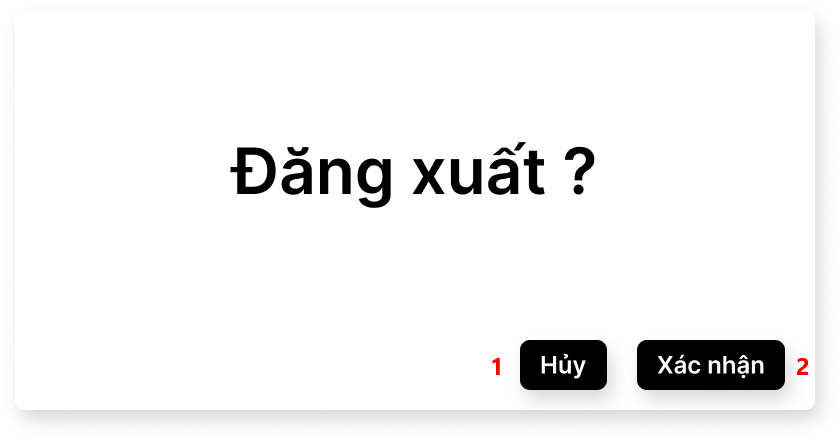
\includegraphics[width=\textwidth]{imgs/mockup/Confirmation pop-up logout.png}
            \captionof{figure}{UI trang quản lý công nhân}
        \end{minipage}
        \hspace{0.05\textwidth}
        \begin{minipage}{0.45\textwidth}
            \begin{tblr}{
                width=1\linewidth,
                hlines, 
                vlines,
                colspec={X[-1]X[2]X[7]},
                columns = {valign = m, },
                column{1} = {halign = c},
                row{1} = {halign = c, valign = m, bg = lightgray, fg = black},
                }
                {\textbf{\#}} & \textbf{Type} & {\textbf{Mô tả}} \\
                1 & Button & Hủy\\
                2 & Button & Xác nhận và thực hiện đăng xuất\\
            \end{tblr}
        \end{minipage}

        \noindent \begin{minipage}{0.5\textwidth}
            \vspace{1cm}
            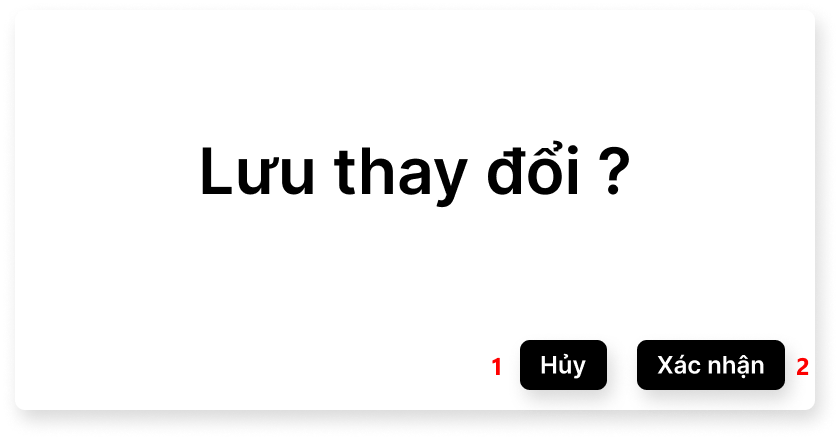
\includegraphics[width=\textwidth]{imgs/mockup/Confirmation pop-up save change.png} 
            \captionof{figure}{UI trang quản lý công nhân}
        \end{minipage}
        \hspace{0.05\textwidth}
        \begin{minipage}{0.45\textwidth}
            \begin{tblr}{
                width=1\linewidth,
                hlines, 
                vlines,
                colspec={X[-1]X[2]X[7]},
                columns = {valign = m, },
                column{1} = {halign = c},
                row{1} = {halign = c, valign = m, bg = lightgray, fg = black},
                }
                {\textbf{\#}} & \textbf{Type} & {\textbf{Mô tả}} \\
                1 & Button & Hủy\\
                2 & Button & Xác nhận và thực hiện lưu thay đổi\\
            \end{tblr}
        \end{minipage}